


\documentclass[11pt, a4paper]{article}



% Loads required packages from the separate file 
%\input{general.tex} 
%% Useful packages
\usepackage{amsmath}
\usepackage{graphicx}
\usepackage[colorinlistoftodos]{todonotes}
\usepackage[colorlinks=true, allcolors=blue]{hyperref}
\usepackage{float}
\usepackage{enumerate}
\usepackage{subfig}



%---------------------------------------------------------------------------------
%General information
%---------------------------------------------------------------------------------
\title{Modeling of the Population Growth Curve} 
\author{Zongyi Hu}
\date{\small \today}




%---------------------------------------------------------------------------------
%	Begin my document
%---------------------------------------------------------------------------------

\begin{document}
% uncomment, if add a cover page"\input{content/0A-coverpage}" and comment "\maketitle" as well as "\input{content/0B-disclaimer}"

\maketitle % uncomment if want a cover page 
%\input{content/0A-coverpage} % Adds a cover page; comment if want a cover page
%\input{content/0B-disclaimer} % Gives you the word count; comment if want a cover page 
%\input{content/0C-toc} % Adds a table of content; uncomment if required

\begin{abstract}
    The sigmoidal curve has extensive application in the real world. With some complex system lacking a specific model, it can be used\cite{gibbs2000variational}. In ecology, specifically, population growth is a typical application. Most cases, the curve will have successive lag, growth, and asymptotic phases. After it gets the asymptote phase which population size has gotten the K value, some data’s population size will drop, which circumstance will not be discussed in the article. In this project, I used computational based methods analysed three models: polynomial(cubic) model, logistic model and Gompertz model. After fitting 285 data sets, the result shows that the Gompertz model performs better than the other two models. +(Succinct discussion).
\end{abstract}


% Introduction
\section{Introduction}
  This article analysed the population (log)size against time. Addressed the basic steps choosing the Cubic, Logistic and Gompertz models\cite{zwietering1990modeling}, basically by comparing $AIC$ and $R^2$.
  
  
% Methods
\section{Methods}
\subsection{Computing tools}
Computational based model fitting project: git, R, python…

\subsection{Data}

285 data set were analysed in this article 

\subsection{Models}
The polynomial, logistic and Gompertz model were chose to fit the data, and comparing the model by calculating $AIC$ and $R^2$. To capture the lag phase, more complicated growth models, the Gompertz model\cite{zwietering1990modeling}, has been chosen in this project, which is asymmetrical compared with the logistic model. The equation of the models I used will be listed bellow: (which t is time, $N_t$ and $N_0$ are the population size at time t and time 0 respectively, $N_max$ is plateau population size, r is growth rate)

\begin{enumerate}[1)]

\item Polynomial Model
\begin{equation*}
 N_t = a + bt + ct^2 + dt^3
\end{equation*}

\item Logistic Model
\begin{equation*}
 N_t= \frac{N_0Ke^{rt}}{K + N_0({e^{rt}-1})}\\
\end{equation*}

\item Gompertz Model
\begin{equation*}
 N_t= N_0 + (N_{max} - N_0) e^{-e^{r_{max} exp^{(1)} {\frac{t_{lag}-t}{(N_{max}-N_0)log(10)}\\} +1}} 
\end{equation*}

\end{enumerate}


\subsection{Model fitting}



% Results
\section{Results}
The Gompertz model performs better than the other two models in this project
\begin{figure}[H]\centering
  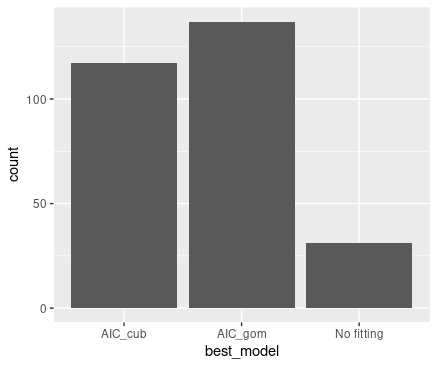
\includegraphics[width=1\textwidth]{best_model_AIC.png}
  \caption{\label{foto1}The frequency of the best model}
  \end{figure}

%Discussion
\section{Discussion}

  

 \bibliographystyle{plain}
  \bibliography{BibMiniPro}


%---------------------------------------------------------------------------------

\end{document}
